\documentclass[12pt]{article}
\usepackage[a4paper]{geometry}
\usepackage[utf8]{inputenc}
\usepackage{fancyhdr}
\usepackage{lastpage}
\usepackage{graphicx, wrapfig, subcaption, setspace, booktabs}
\usepackage{graphicx}
\usepackage[T1]{fontenc}
\usepackage[font=small, labelfont=bf]{caption}
\usepackage[protrusion=true, expansion=true]{microtype}
\usepackage[english]{babel}
\usepackage{sectsty}
\usepackage{url, lipsum}
\usepackage[T1]{fontenc}
\usepackage{icomma}
\usepackage{siunitx}
\usepackage{ragged2e}
\usepackage{amsmath}
\usepackage{comment}
\usepackage{enumerate}
\usepackage{anysize}
\usepackage{graphicx}
\usepackage{amssymb}
\usepackage{apacite}
\bibliographystyle{apacite}
\newcommand{\HRule}[1]{\rule{\linewidth}{#1}}
\onehalfspacing
\setcounter{tocdepth}{5}
\setcounter{secnumdepth}{5}
\usepackage[utf8]{inputenc}
\usepackage{amssymb}
\usepackage{graphicx}
\usepackage{amsmath}
\onehalfspacing
\setcounter{tocdepth}{5}
\setcounter{secnumdepth}{5}

%-------------------------------------------------------------------------------
% HEADER & FOOTER
%-------------------------------------------------------------------------------


\begin{comment}
-Udledninger
$$
\begin{aligned}
\end{aligned}
$$

-Opgavetekst
\begin{figure}[H]
\includegraphics[width=0.5\textwidth]{"path"}
\end{figure} 


-Opgave billede med tekst
\begin{figure}[H]
\caption{"Billedtekst"}
\includegraphics[width=0.5\textwidth]{"path"}
\end{figure} 

-Værdier
$\\
$


\end{comment}
\begin{document}

\begin{titlepage}

\title{ \normalsize 
		%\begin{figure}
        \begin{center}
        
\includegraphics[height=6cm]{Logo.jpg}
        \end{center}
       % \end{figure}
        \LARGE \textsc{\textbf{Universidad De Sonora}} \\ \bigskip
		\Large División de Ciencias Exactas y Naturales \\
        Licenciatura en Física \\ \bigskip
        \bigskip
        Física Computacional I
		\\ [0.1cm]  
		\HRule{2pt} \\
		\Large \textbf{{Actividad 11}} \\
        \textit{\textbf{"Solución Numérica de la Ecuación de Onda."}}
		\HRule{2pt} \\
		\normalsize \vspace*{0.001\baselineskip}}
        
\date{\bigskip \Large  \hspace*{\fill} Hermosillo, Sonora a abril 15 de 2021}

        
\author{
		\Large\textbf{Ismael Espinoza Arias} \\ \bigskip
        \\ \bigskip
       \Large Profesor Carlos Lizárraga Celaya}
       \end{titlepage}
       \maketitle
       
       
%-----------------------------------------------------------


\section{Ecuación de onda}

Consideremos una perturbación, generada en una cuerda, que viaja hacia
la derecha con una rapidez constante u. Si convenimos en denotar por x
a las diferentes posiciones a lo largo de la dirección de propagación de la
perturbación y por y a las posiciones perpendiculares a ésta, la forma de la
perturbación quedará descrita por una función y = f(x,t). Si durante la propagación
de la perturbación no existe disipación de energía, la forma y el tamaño de la
perturbación no cambiarán a medida que ésta se desplaza. (En particular, la
propagación de la luz en el espacio vacío cumple con este requisito.) En tal caso
se debe cumplir necesariamente que:

\begin{center}
    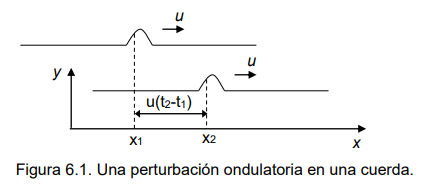
\includegraphics[height=6cm]{E1.png}
\end{center}

en donde $x2 = x1 + u(t2 - t1), ya que u(t2 - t1)$ es la distancia que ha avanzado la
perturbación en el intervalo t2 - t1. Este requisito se cumple si la función que
describe a la perturbación tiene la forma:

\begin{center}
    $f(x,t) = y(x - ut) $
    
    ya que entonces:
    
    $f(x2,t2) = y(x2 - ut2) = y[x1 + u(t2 - t1)- ut2] = y( x1 - ut1) = f(x1,t1)$
    
\end{center}

La ecuación de onda es una ecuación diferencial parcial de segundo orden en el tiempo y las coordenadas espaciales y tiene la forma

\begin{equation*}
\frac{\partial^2 u}{\partial t^2} = c^2 \left( 
  \frac{\partial^2 u}{\partial x^2} +
  \frac{\partial^2 u}{\partial y^2} +
  \frac{\partial^2 u}{\partial z^2} \right) + f(x,y,z,t)
\end{equation*}

donde $c^{2}$ es la velocidad de propagación de la información. La función $u(x,y,z,t)$ representa la presión en una onda acústica, la intensidad de un campo electromagnético, el desplazamiento respecto a un nivel de referencia como lo puede ser la amplitud de una onda superficial en la superficie del agua o el desplazamiento respecto a la horizontal de una cuerda vibrante. 

En una dimensión, por ejemplo el caso de una cuerda vibrante, la Ecuación de Onda se simplifica a 

\begin{equation*}
\frac{\partial^2 u}{\partial t^2} = c^2 \left( 
  \frac{\partial^2 u}{\partial x^2}
   \right) + f(x,t) \qquad x \in (0,L], t \in (0,T]
\end{equation*}

Requerimos definir 4 condiciones: 2 iniciales (derivada de segundo orden en t) y 2 a la frontera (segundo orden en el espacio), para encontrar la solución.

\begin{eqnarray*}
u(x,0) & = & I(x) \\
\frac{\partial}{\partial t} u(x,0) & = & 0 \\
u(0,t) & = & 0 \\
u(L,t) & = & 0 \\
\end{eqnarray*}

Se requiere también especificar el valor de la constante $c$ y la función $I(x)$.



%-----------------------------------------------------------


\section{Solución de la Ecuación de Onda en una dimensión por el Método de Diferencias Finitas.}

Podemos comenzar aproximando las segundas derivadas por diferencias finitas centradas de segundo orden.

Si $h$ es el incremento en la dirección $x=\Delta x$ y $k=\Delta t$ es el incremento en el tiempo. Entonces en un punto de la malla discreta $(x,t)$ tendremos

\begin{equation*}
\frac{u(x,t+k) -2u(x,t) + u(x,t-k)}{k^2} = c^2
\frac{u(x+h,t) -2u(x,t) + u(x-h,t)}{h^2}
\end{equation*}

La ecuación anterior define un esténcil computacional de 5 puntos y se respresenta como:

\begin{center}
    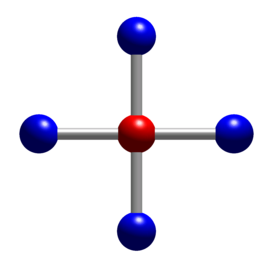
\includegraphics[height=6cm]{E2.png}
\end{center}


%-----------------------------------------------------------


\subsection*{Importación de bibliotecas}
Empezamos importando nuestras bibliotecas, el primer paso para empezar con cualquier actividad.

\begin{center}
    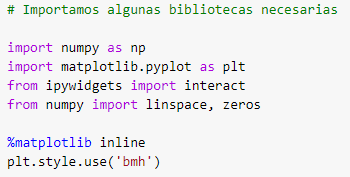
\includegraphics[height=6cm]{bibliotecas.png}
\end{center}
 
 Donde podemos ver que las bibliotecas utilizadas, son numpy, scipy, matplotlib, toolkits, ect. Donde nos ayudaran a resolver nuestro siguiente problema.


%-----------------------------------------------------------


\subsection*{Realización de la actividad}
Ahora para la actividad, vamos a definir nuestros valores y resolver la ecuación de onda usando ecuaciones diferenciales parciales.

\begin{center}
    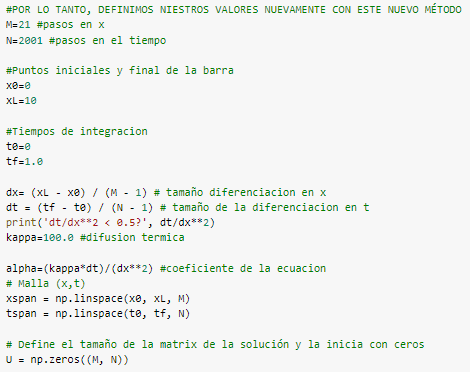
\includegraphics[height=10cm]{E3.png}
    \includegraphics[height=10cm]{cuerda.png}
\end{center}

 

%--------------------------1---------------------------------


\subsection*{Ejercicio 1}

Modifique el algoritmo de diferencias finitas empleado anteriormente y resuelva la ecuación de onda amortiguada en una dimensión, dada por la ecuación

\begin{equation*}
\frac{\partial^2 u}{\partial t^2} + 
 b \frac{\partial u}{\partial t}
 = c^2 \left( 
  \frac{\partial^2 u}{\partial x^2}
   \right) \qquad x \in (0,L], t \in (0,T]
\end{equation*}

donde $b \ge 0 $ y $c$ son constantes. 

Se proporcionan las condiciones iniciales y a la frontera para encontrar la solución.

\begin{eqnarray*}
u(x,0) & = & I(x) \\
\frac{\partial}{\partial t} u(x,0) & = & 0 \\
u(0,t) & = & 0 \\
u(L,t) & = & 0 \\
\end{eqnarray*}

Utilice diferencias finitas centradas de segundo orden para aproximar la primer derivada $\partial u/\partial t$.

\begin{equation*}
\frac{\partial}{\partial t} u(x,t) \approx \frac{u(x,t+k) - u(x,t-k)}{2k}
\end{equation*}

Suponga las mismas características del ejemplo presentado anteriormente $L=10$, $c=100$m/s, $t=(0,0.25)$, y coeficiente de amortiguamiento $b=0.5$ con condiciones iniciales $u(x,0) = x(1-x)$ y $\partial u(x,0) / \partial t = 0$ y condiciones a la frontera $u(0,t)=u(L,t)=0$. 

Realizamos la resolución de nuestro ejercicio.

\begin{center}
    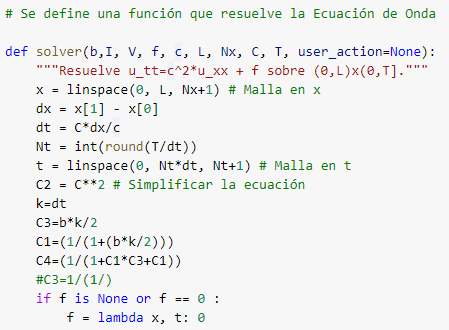
\includegraphics[height=10cm]{E4.png}
    
    Donde llegamos al siguiente resultado:
    
    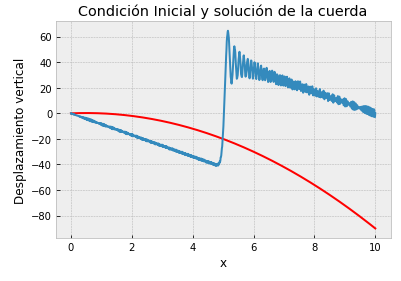
\includegraphics[height=8cm]{Ejercicio1.png}
\end{center}




%---------------------------2--------------------------------


\subsection*{Ejercicio 2}

Haga el desarrollo del algoritmo de diferencias finitas centradas para resolver la ecuación de onda en 1 dimensión si se tiene un término de forzamiento $f(x,t)$

\begin{equation*}
\frac{\partial^2 u}{\partial t^2} = c^2 \left( 
  \frac{\partial^2 u}{\partial x^2}
   \right) + f(x,t) \qquad x \in (0,L], t \in (0,T]
\end{equation*}

Con las condiciones iniciales y a la frontera para encontrar la solución.

\begin{eqnarray*}
u(x,0) & = & I(x) \\
\frac{\partial}{\partial t} u(x,0) & = & 0 \\
u(0,t) & = & 0 \\
u(L,t) & = & 0 \\
\end{eqnarray*}

Realizamos la resolución de nuestro ejercicio.

\begin{center}
    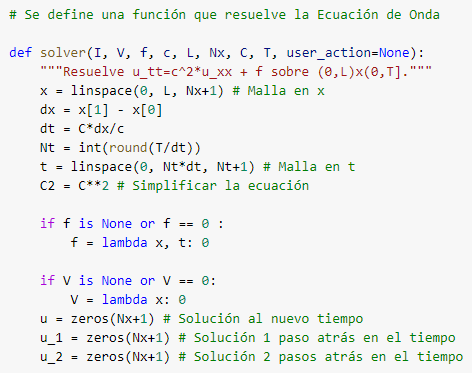
\includegraphics[height=10cm]{Ejercicio2.png}
    
    Donde llegamos al siguiente resultado:
    
    \includegraphics[height=8cm]{Ejercicio2.1.png}
\end{center}


%---------------------------3---------------------------------


\subsection*{Ejercicio 3}

Resuelva la Ecuación KdV, para el caso de 2 solitones comenzando en $x01 = 0.25*L$ y $x02 = 0.75*L$, con velocidades $c1=0.75$ y $c2=0.01$ e integre hasta que una de las ondas llegue a la frontera.

Grafique las soluciones como en el ejemplo que se proporcionó.


Realizamos la resolución de nuestro ejercicio.

\begin{center}
    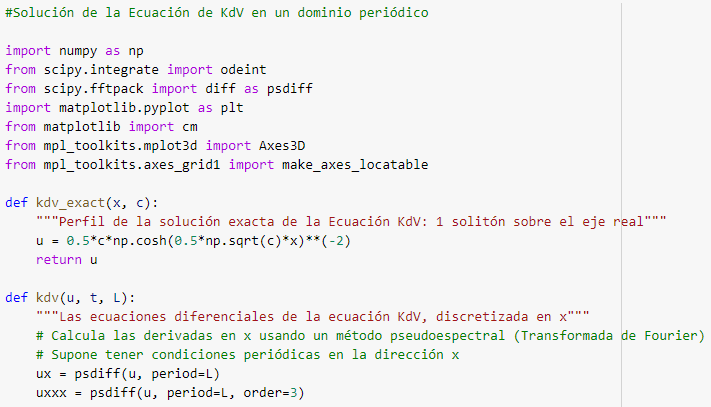
\includegraphics[height=8cm]{Ejercicio3.png}
    
    Donde llegamos al siguiente resultado:
    
    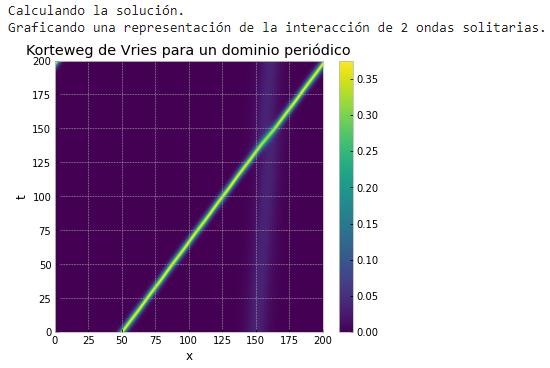
\includegraphics[height=8cm]{Ejercicio3.1.png}
    
     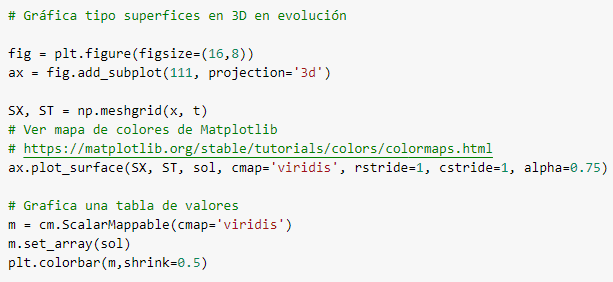
\includegraphics[height=6cm]{Ejercicio3.2.png}
    
    Donde llegamos al siguiente resultado:
    
    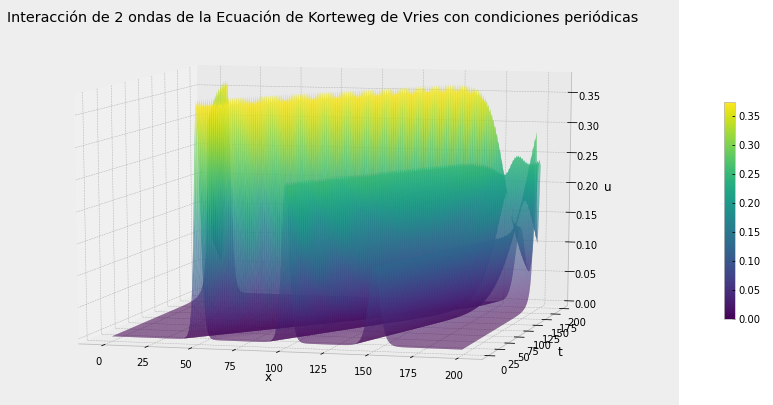
\includegraphics[height=8cm]{Ejercicio3.3.png}
\end{center}


%---------------------------4---------------------------------


\subsection*{Ejercicio 4}

Resuelva la Ecuación KdV, para el caso de 3 solitones comenzando en $x01 = 0.25*L$, $x02=0.5*L$, y $x03 = 0.75*L$, con velocidades $c1=0.75$, $c2=0.5$ y $c3=0.25$ e integre hasta que una de las ondas llegue a la frontera.

Grafique las soluciones.

Realizamos la resolución de nuestro ejercicio.

\begin{center}
    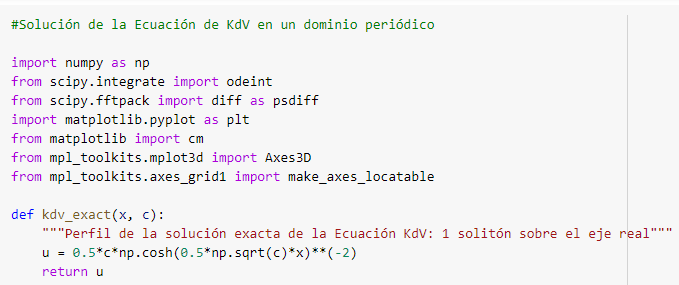
\includegraphics[height=6cm]{Ejercicio4.png}
    
    Donde llegamos al siguiente resultado:
    
    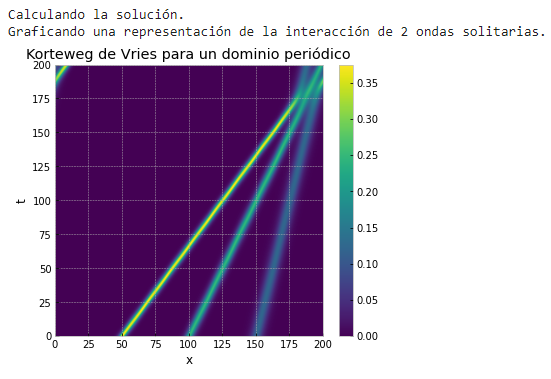
\includegraphics[height=8cm]{Ejercicio4.1.png}
    
     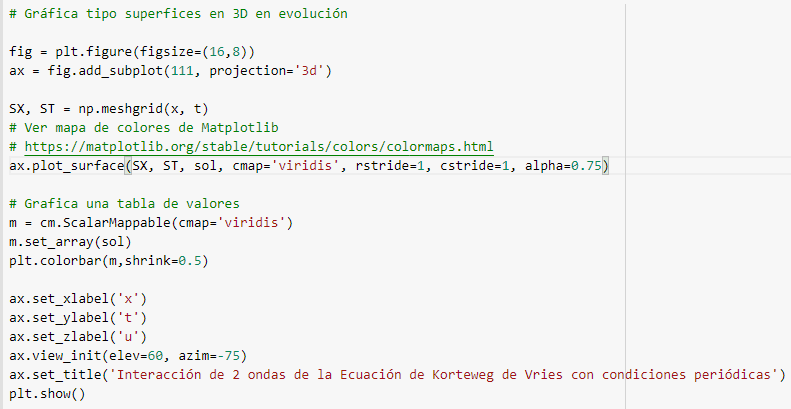
\includegraphics[height=8cm]{Ejercicio4.2.png}
    
    Donde llegamos al siguiente resultado:
    
    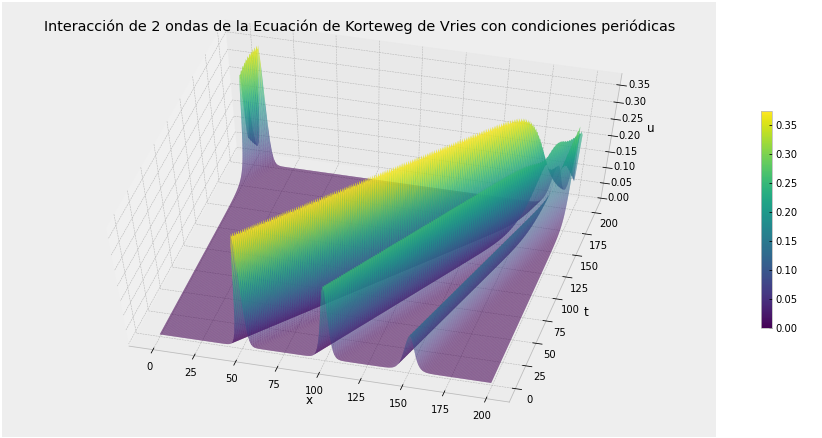
\includegraphics[height=8cm]{Ejercicio4.3.png}
\end{center}


%---------------------------5---------------------------------


\subsection*{Ejercicio 5}

En el ejemplo resuleto anterior, se mostró la evolución de la condición inicial 

\begin{equation*}
u_0^{(2,1)}(x,y,0) = sin (\pi x) \sin (\frac{\pi y}{2})
\end{equation*}

mostrando el *modo (1,2)* de oscilación natural de la membrana ([Ver estas animaciones](https://www.acs.psu.edu/drussell/Demos/MembraneSquare/Square.html)). 
 
En este Ejercicio se pide mostrar la evolución del *modo (1,1)*, con la condición inicial 

\begin{equation*}
u_0^{(1,1)}(x,y,0) = \sin (\frac{\pi x}{2}) \sin (\frac{\pi y}{2})
\end{equation*}

\begin{center}
    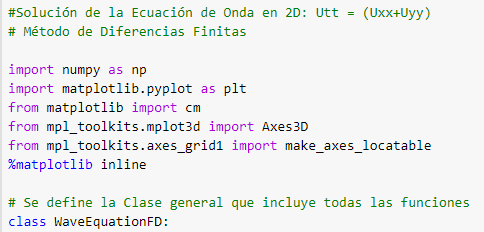
\includegraphics[height=6cm]{Ejercicio5.png}
    
    Donde llegamos a la siguientes gráficas:
    
    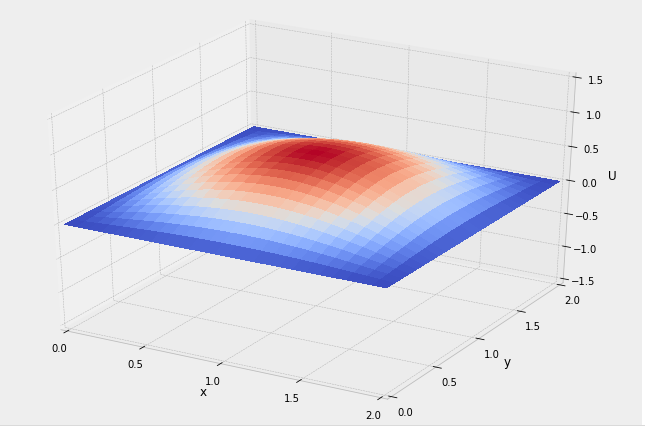
\includegraphics[height=5cm]{Gráfica1.png}
    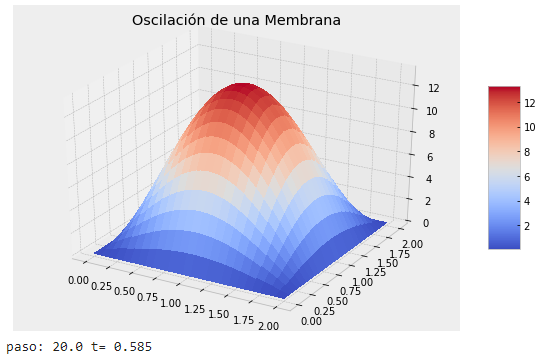
\includegraphics[height=5cm]{Gráfica2.png}
    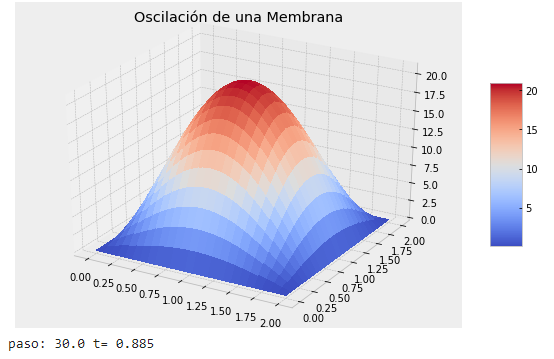
\includegraphics[height=5cm]{Gráfica3.png}
    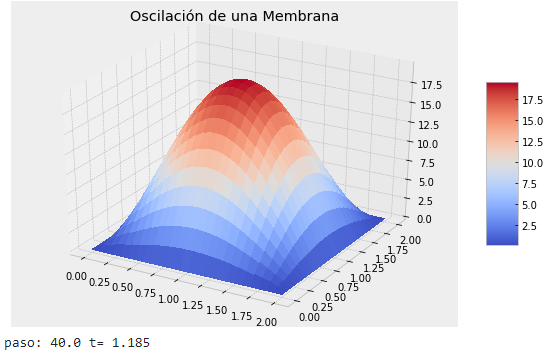
\includegraphics[height=5cm]{Gráfica4.png}
    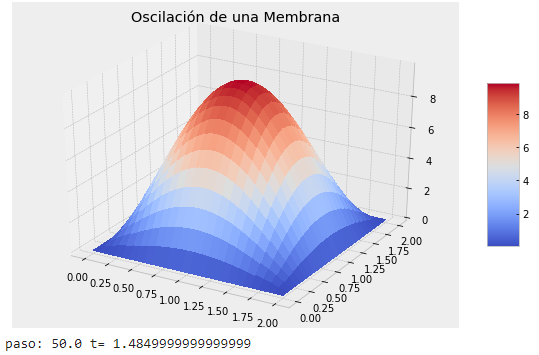
\includegraphics[height=5cm]{Gráfica5.png}
    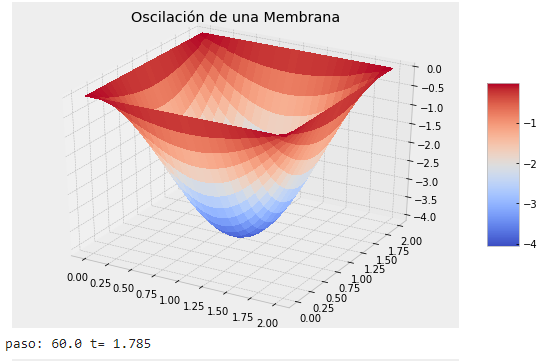
\includegraphics[height=5cm]{Gráfica6.png}
    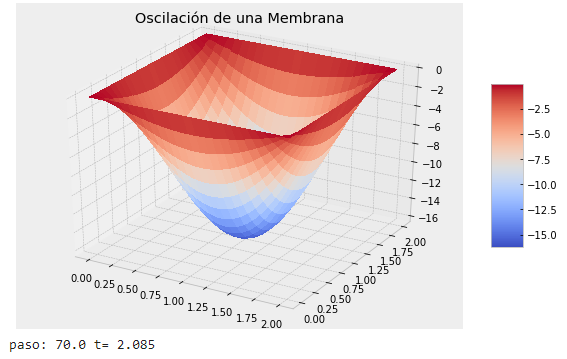
\includegraphics[height=5cm]{Gráfica7.png}
    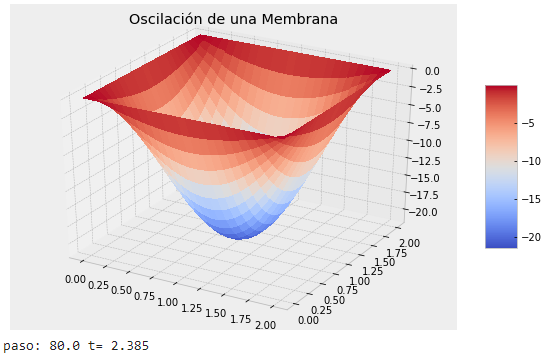
\includegraphics[height=5cm]{Gráfica8.png}
    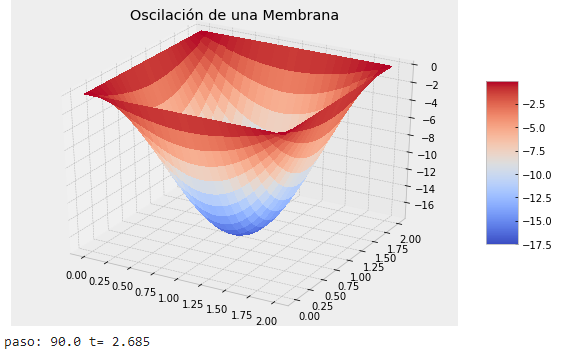
\includegraphics[height=5cm]{Gráfica9.png}
    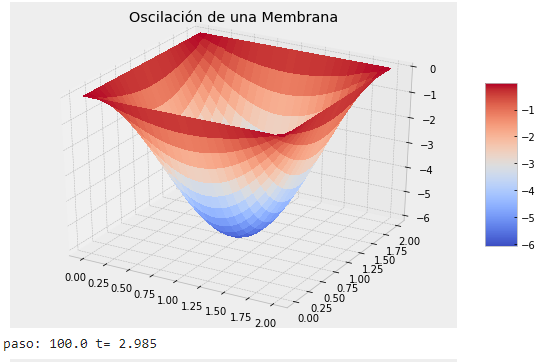
\includegraphics[height=5cm]{Gráfica10.png}
    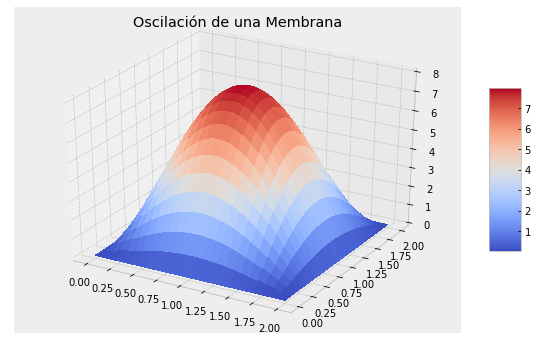
\includegraphics[height=5cm]{Gráfica11.png}
    
\end{center}


%---------------------------6---------------------------------


\subsection*{Ejercicio 6}

En el mismo contexto que el problema anterior, muestra la evolución de la superposición *modos (3,1)+ (1,3)* dada la condición inicial

\begin{equation*}
u_0^{(3,1)+(1,3)}(x,y,0) = \sin (\frac{3 \pi x}{2}) \sin (\frac{\pi y}{2}) + \sin (\frac{\pi x}{2}) \sin (\frac{3 \pi y}{2})
\end{equation*}

\begin{center}
    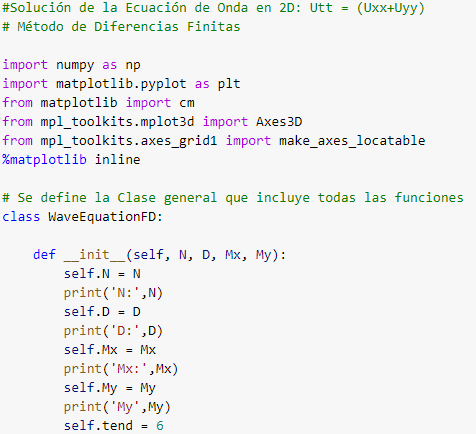
\includegraphics[height=10cm]{Ejercicio6.png}
    
    Donde llegamos a la siguientes gráficas:
    
    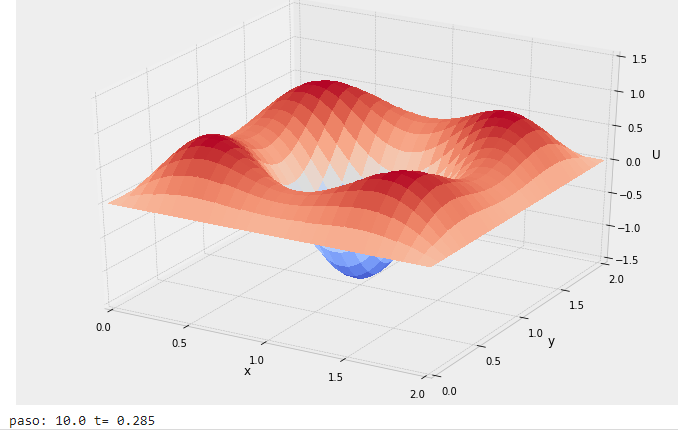
\includegraphics[height=5cm]{s1.png}
    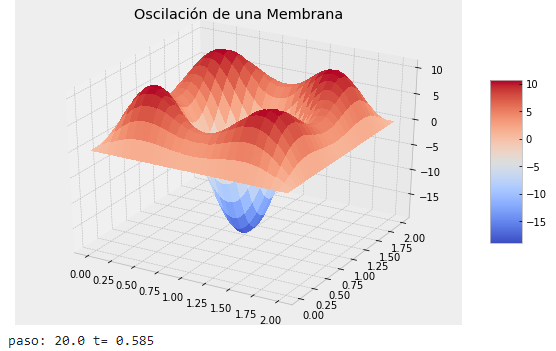
\includegraphics[height=5cm]{s2.png}
    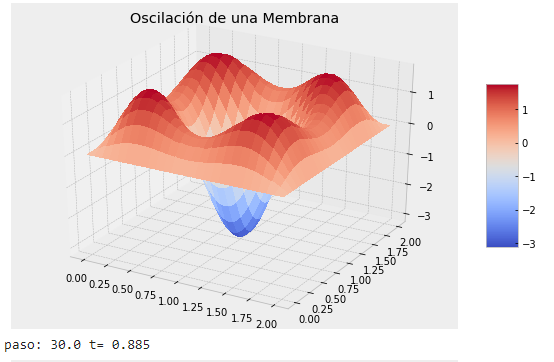
\includegraphics[height=5cm]{3.png}
    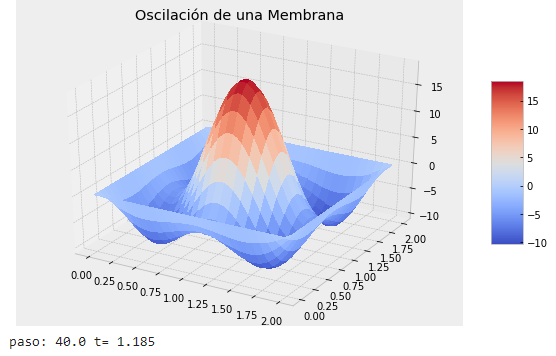
\includegraphics[height=5cm]{s4.png}
    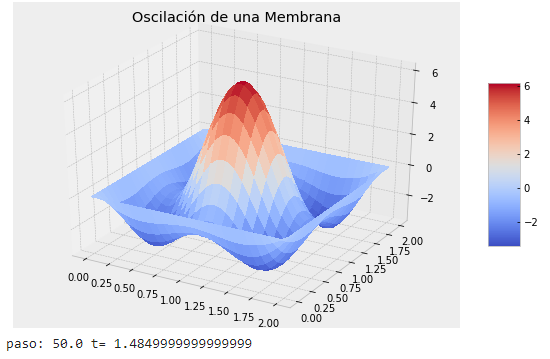
\includegraphics[height=5cm]{s5.png}
    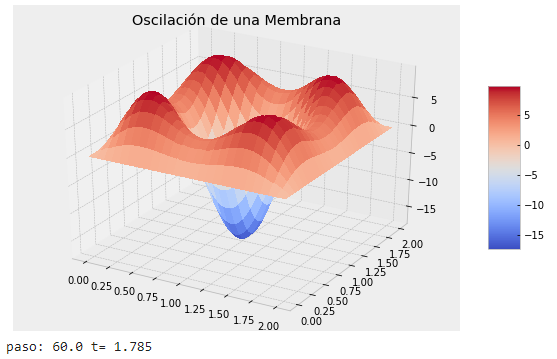
\includegraphics[height=5cm]{s6.png}
    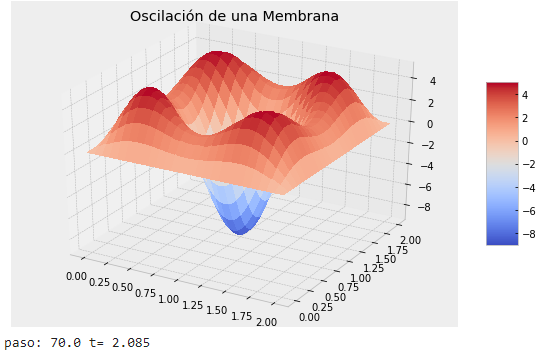
\includegraphics[height=5cm]{s7.png}
    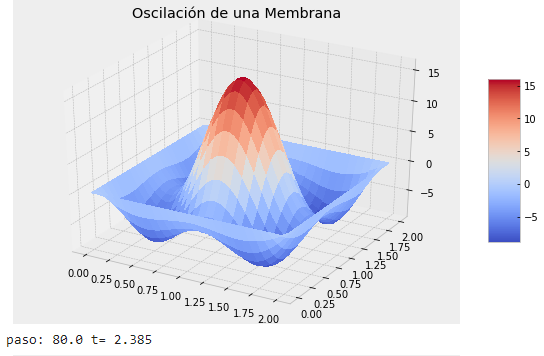
\includegraphics[height=5cm]{s8.png}
    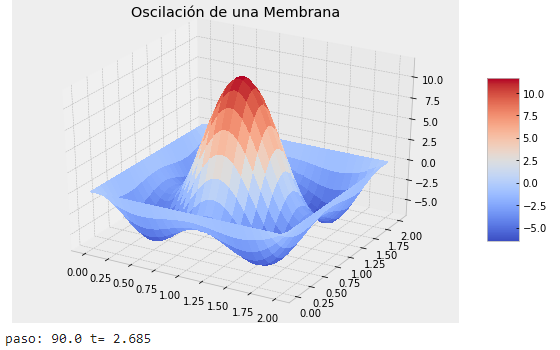
\includegraphics[height=5cm]{s9.png}
    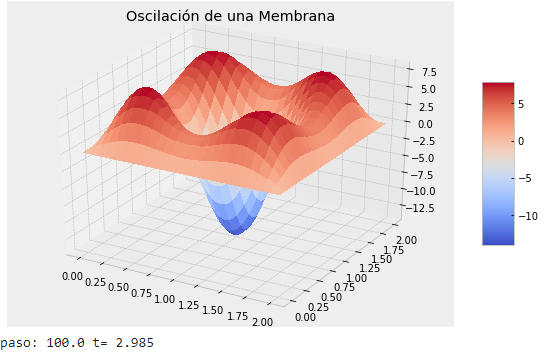
\includegraphics[height=5cm]{s10.png}
    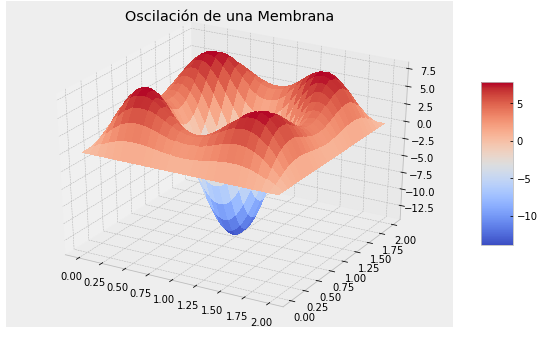
\includegraphics[height=5cm]{s11.png}

    
\end{center}
\newpage

\section*{Conclusiones, resultados y discusión}
En esta activiadad se reforzaron los conocimientos adquridos en las clases de teoría, impartidas por el docente en el transcruso de la semana. En esta ocasión resolvimos y aplicamos algunos ejemplos de la ecuación de calor, donde graficamos las soluciones viendo como es que estas se comportan. También vimos 2 métodos aplicamos para realizar este ejercicio y de una forma utilizando las diferencias finitas.


%-----------------------------------------------------------



\section*{Bibliografía}
\begin{itemize}

\item \textit{Wave Equation. (s. f.). Hyperphysics. Recuperado 21 de abril de 2021, de http://hyperphysics.phy-astr.gsu.edu/hbasees/Waves/waveq.html}

\item \textit{Tomé, C. (2018, 20 noviembre). Fase y ecuación de onda. Cuaderno de Cultura Científica. https://culturacientifica.com/2018/11/20/fase-y-ecuacion-de-onda/.}

\item \textit{Ecuación de Onda. (s. f.). Ecuación de Onda. Recuperado 21 de abril de 2021, de https://www.compadre.org/osp/EJSS/4446/240.htm.}

\end{itemize}


%-----------------------------------------------------------


\section*{Apéndice}
\begin{enumerate}

\item ¿Qué aprendiste nuevo?\\
\textit{Aprendí como se resulve la ecuación de calor con el uso de difrencias finitas y aplicaciones y gráficas que llaman la atención visualmente.}

\item ¿Qué fue lo que más te llamó la atención de la ecuación del calor?\\
\textit{Su resolución, ya ecuaciones diferenciales parciales aplicadas en un campo específico me gustan y me llaman mucho la atención, es por eso que como la ecuación de onda se resuelve de esta forma, me gusta.}

\item ¿Qué mejorarías en esta actividad?\\
\textit{Tratar de referenciar con información mas digerible rapidamente, podria decir.}

\item ¿Algún comentario adicional antes de dejar de trabajar en Jupyter con Python?\\
\textit{Es un lenguaje de los más usados y muy extenso, pero presiento que conocí una parte valiosa de él.}

\item Cerramos la parte de trabajo con Python ¿Que te ha parecido?\\
\textit{Fue una buena experiencia trabajar con este lenguaje, pues, es muy fácil de manejar a diferencia de otros, y logra cosas que otros no pueden o bien sea una tarea dificil, tal es el caso de métodos numéricos, graficación, solución de sistemas de ecuaciones diferenciales, etc. Todo con la ayuda de sus bibliotecas.}

\end{enumerate}

\end{document}